%\documentstyle[11pt,a4]{article}
%\documentclass[a4paper]{article}
\documentclass[a4paper, 10pt]{article}
% Seems like it does not support 9pt and less. Anyways I should stick to 10pt.
%\documentclass[a4paper, 9pt]{article}
\topmargin-2.0cm

\usepackage{fancyhdr}
\usepackage{pagecounting}
\usepackage[dvips]{color}
\usepackage{wrapfig}
\usepackage{graphicx}
\usepackage{hyperref}

% Color Information from - http://www-h.eng.cam.ac.uk/help/tpl/textprocessing/latex_advanced/node13.html

% NEW COMMAND
% marginsize{left}{right}{top}{bottom}:
%\marginsize{3cm}{2cm}{1cm}{1cm}
%\marginsize{0.85in}{0.85in}{0.625in}{0.625in}

\def\ie{{\em i.e.,}}
\def\eg{{\em e.g.,}}
\newcommand{\tabref}[1]{Table~\ref{#1}}
\newcommand{\figref}[1]{Figure~\ref{#1}}
\newcommand{\secref}[1]{Section~\ref{#1}}

\advance\oddsidemargin-0.65in
%\advance\evensidemargin-1.5cm
\textheight9.2in
\textwidth6.75in
\newcommand\bb[1]{\mbox{\em #1}}
\def\baselinestretch{1.05}
%\pagestyle{empty}

\newcommand{\hsp}{\hspace*{\parindent}}
\definecolor{gray}{rgb}{0.4,0.4,0.4}
%\definecolor{gray}{rgb}{1.0,1.0,1.0}


\begin{document}
\thispagestyle{fancy}
%\pagenumbering{gobble}
%\fancyhead[location]{text} 
% Leave Left and Right Header empty.
\lhead{}
\rhead{}
%\rhead{\thepage}
\renewcommand{\headrulewidth}{0pt} 
\renewcommand{\footrulewidth}{0pt} 
\fancyfoot[C]{\footnotesize \textcolor{gray}{\href{https://norouzi.github.io/}{https://norouzi.github.io/}}} 

%\pagestyle{myheadings}
%\markboth{Sundar Iyer}{Sundar Iyer}

\pagestyle{fancy}
\lhead{\textcolor{gray}{\it Mohammad Norouzi}}
\rhead{\textcolor{gray}{\thepage/\totalpages{}}}
%\rhead{\thepage}
%\renewcommand{\headrulewidth}{0pt} 
%\renewcommand{\footrulewidth}{0pt} 
%\fancyfoot[C]{\footnotesize http://www.stanford.edu/$\sim$sundaes/application} 
%\ref{TotPages}

% This kind of makes 10pt to 9 pt.
%\begin{small}

%\vspace*{0.1cm}
\begin{center}
{\LARGE \bf Research Statement}\\
\vspace*{0.1cm}
{\normalsize Mohammad Norouzi (mnorouzi@google.com)}
\vspace*{0.2cm}
\end{center}
%\vspace*{0.2cm}

%\begin{document}
%\centerline {\Large \bf Research Statement for Mohammad Norouzi}
%\vspace{0.5cm}

% Write about research interests...
%\footnotemark
%\footnotetext{Check This}


My research lies in {\em Machine Learning (ML)} with applications
to {\em Computer Vision} and {\em Natural Language Processing
  (NLP)}. I study the mathematical principles and statistical modeling
assumptions that can lead to the emergence of {\em Artificial
  Intelligence (AI)}.  I believe there exists a class of simple and
universal algorithms that can successfully address many challenging ML
problems. Hence, my research aims to develop simple and generic ML
algorithms that are broadly applicable across a range of problem
domains including computer vision and NLP. I am interested in bridging
the gap between existing ML formulations (see~\cite{raml,pcl}) to
help simplify and unify common ML objective functions and investigate
the benefits and weaknesses of each approach. My research makes heavy
use of {\em deep neural networks} because of their flexibility and
effectiveness (\eg~\cite{seq2seq,alphago}) and attempts to make neural
networks even more powerful and widely applicable.

%% \begin{wrapfigure}{r}{2in}
%% %\begin{figure}
%% \vspace*{-.2cm}
%%   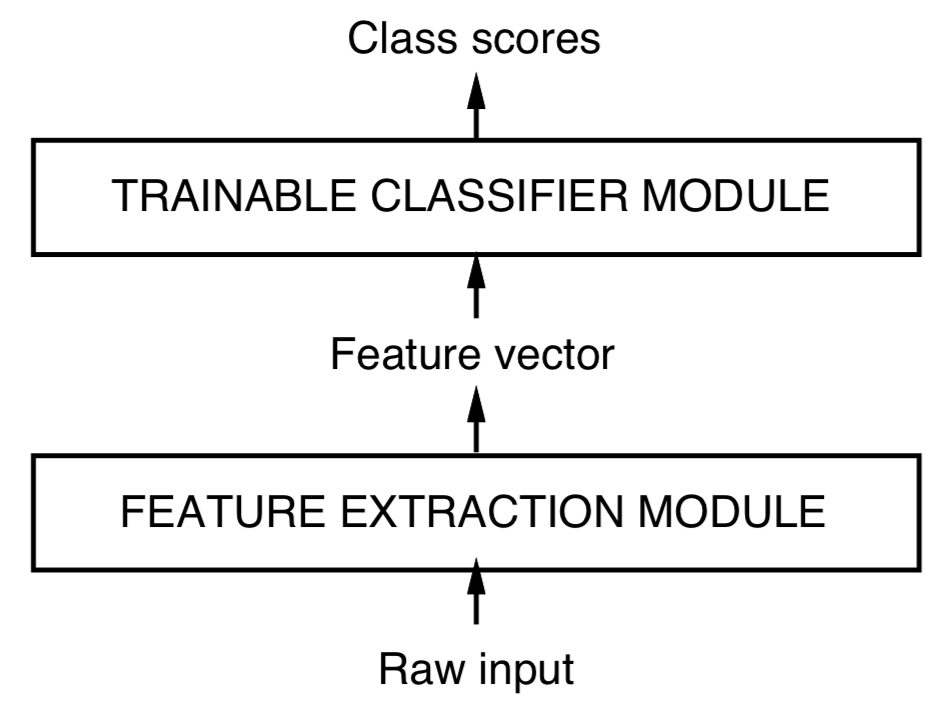
\includegraphics[width=2in]{fig1.png}
%% \vspace*{-.2cm}
%%   \caption{\small Figure from \cite{lecun98}, which highlights the
%%     inefficiency of traditional pattern recognition with separately
%%     tuned feature extraction and classification modules.}
%%   \label{fig:fig1}
%% \end{wrapfigure}
%(\eg~\figref{fig:fig1}).

My current research aims to enable effective and efficient {\em
  end-to-end} optimization of multi-stage pipelines that involve {\em
  discrete} latent variables and {\em non-differentiable} components.
I am inspired by the success of error back propagation through
multilayer neural networks to jointly optimize hierarchical feature
extraction and classification modules~\cite{backprop,lecun98}.  My
research aspires to facilitate goal driven joint optimization of
complex AI systems, which comprise vision, natural language, memory,
and reasoning modules. I believe by adopting an end-to-end
optimization approach, one can achieve higher degree of efficiency and
effectiveness compared to hand engineered pipelines.  For example, my
previous work has demonstrated the effectiveness of (1) end-to-end
optimization of metric learning and quantization
modules~\cite{mlh,hdml}, (2) non-greedy optimization of decision
trees~\cite{engodt}, (3) joint optimization of keypoint extraction and
pose estimation modules~\cite{keypointnet}, and (4) goal-driven
optimization of sequence models based on a sequence level reward
feedback~\cite{mapo,ocd}. Generally, end-to-end optimization based on
a well defined objective function offers a principled way to fine-tune
multi-stage pipelines and encourages effective cooperation among
different modules.

\vspace*{-.2cm}
\subsubsection*{End-to-end Stochastic Optimization of Discrete Latent Variables}
\vspace*{-.1cm}

\hspace{\parindent} {\em Discrete} latent variables are ubiquitous in
machine learning models that utilize mixture of experts, efficient
lookup tables~\cite{mih}, hard attention~\cite{hardattention}, and
structured outputs. Using discrete variables as intermediate ML
representations often facilitates {\em interpretability} and improves
{\em efficiency}. For example, consider a question answering system
that needs to convert natural language questions to output
answers. One can optimize a neural network to directly perform this
mapping, or alternatively, one can train a neural network to first
generate an intermediate SQL program, and then execute such a program
on a database to obtain the final answer~\cite{mapo}. Having access to
the underlying latent programs allows one to gain insights into the
inner workings of the question answering system. For example, this
would allow one to attribute an incorrect answer to either an issue in the
database or in the model's understanding of the
question. Interpretability is especially important for sensitive
application areas such as medicine and public policy. Nevertheless,
end-to-end optimization of discrete variables is challenging due to
lack of {\em differentiability}.

To differentiate through discrete latent variables, I advocate the use
of a stochastic relaxation of the objective functions in terms of an
expectation {\em w.\,r.\,t.}~a distribution over discrete
variables. For example, to optimize over latent programs, one can
maximize an expectation of a score function per program, where the
expectation is {\em w.\,r.\,t.}~a parametric distribution over all
possible programs.  Then, one can adopt ideas from {\em Reinforcement
Learning (RL)} and policy optimization~\cite{sutton1998reinforcement}
to optimze the stochastic objective function. We have applied the
REINFORCE algorithm~\cite{reinforce} and its variants to structured
output prediction~\cite{wu2016gnmt} and combinatorial optimization
with discrete structures~\cite{bello2016neural,azalia2017}. While this
approach to end-to-end optimization of discrete variables is
promising, a key limitation stems from the high variance of gradient
estimates because of Monte Carlo sampling.

A key theme in my research has been trying to bridge the gap between
policy optimization and supervised learning to avoid using high
variance gradient estimates (see~\cite{raml,pqt2018,ocd,dvn,mapo}).
In our recent work, we present Memory Augmented Policy Optimization
(MAPO)~\cite{mapo} as a way to incorporate off-policy trajectories to
reduce the variance of policy gradient estimates without introducing
any bias. MAPO achieves the state-of-the-art results in weakly
supervised semantic parsing. The independent work of Lieu {\em et
  al.}~\cite{liu2018rao} extends the application of MAPO to generative
models with discrete latent variables. Current formulation of MAPO is
limited to deterministic score functions, which makes this algorithm
not suitable for stochastic RL problems. I have developed a
generalization of MAPO based on control variates that makes this
approach more widely applicable, and we are currently performing
experiments on stochastic contextual bandit problems. I am also
planning to incorporate bootstrapping into the formulation of MAPO to
optimize long action trajectories. More generally, I am interested in
bridging the gap between imitation learning and RL algorithms,
extending our previous results~\cite{ocd} to facilitate more effective
optimization of discrete variables within ML.

\vspace*{-.2cm}
\subsubsection*{End-to-end Abstraction of Reinforcement Learning Problems}
\vspace*{-.1cm}

\hspace{\parindent} Pixel observations from RL environments are hardly
interpretable, even though the underlying dynamics are often
simple. One can think of the problem of recovering the underlying MDP
abstraction of an RL problem as another instance of learning discrete
latent representations. For example, consider an Atari game, in which
observations comprise $84\!\times\!84$ color images, while the
underlying dynamics can be defined in terms of relatively simple
rules. In many cases, one does not require access to the full image
observation for planning, but rather the core components of the game
such as locations of the agent, enemies, and obstacles are enough
to define an optimal policy. A key research question is how to
effectively learn an abstract representation of an RL problem to
facilitate efficient planning and exploration. In a recent
paper~\cite{coex}, we have shown that if one automatically discovers
higher level representations based on the position of the controllable
agent, then one can significantly improve performance by more
structured exploration.

From an end-to-end optimization perspective, the best way to evaluate
an abstraction of an RL problem is via examination of such an
abstraction in planning and policy optimization. Given observations
from an RL environment, I intend to automatically extract an MDP
abstraction and use it for planning such that one can differentiate
through the process of MDP abstraction and planning jointly. I would
like to make sure that optimal trajectories in the abstract MDP can be
translated back into near-optimal trajectories in the original
environment. Because the abstract MDP is fully observed, one can find
the optimal policy by efficient value or policy iteration, whereas the
original environment does not comply with such algorithms. An MDP
abstraction comprises a pre-specified number of abstract states, a
transition model between abstract states, and an abstract reward
function. For simplicity, we will assume that the abstract MDP and the
RL environment share the same set of possible actions. Furthermore, we
need a stochastic mapping from observations of the RL environment to
states of the abstract MDP. An important benefit of this approach is
that given the structure of the abstract MDP, one can {\em interpret} a
policy by visualizing the abstract state transitions and by clustering
the observations that represent the same abstract state.

\vspace*{-.2cm}
\subsubsection*{End-to-end Geometric Reasoning}
\vspace*{-.1cm}

\hspace{\parindent} Another example of interesting discrete structure
in machine learning is the 3D geometric structure shared by instances
of an object category. In a recent paper~\cite{keypointnet} for
end-to-end optimization of category-specific 3D keypoints, along with
their detectors, for a downstream geometric vision task. Given a
single image, we extract 3D keypoints that are consistent across
viewing angles and instances of the corresponding object category. We
make use of real valued keypoint coordinates for ease of optimization,
but, the difficulty lies in differentiating Through the geometric
reasoning module. We propose a differentiable objective function that
seeks the optimal list of keypoints for recovering the relative pose
between two views of an object, and we rely on differentiating through
Singular Value Decomposition (SVD) for optimization.  Importantly, we
find that our end-to-end geometric reasoning framework using no
ground-truth keypoint annotations outperforms a fully supervised
baseline (using the same neural network architecture) on the task of
pose estimation. I believe we need to come up with better ways of
incorporating 3D geometry into our generative and discriminative
neural networks, and KeypointNet is one step in that direction. I will
continue working on this problem, and inspired by some recent
work~\cite{kanazawa}, I have some concrete ideas to facilitate other
forms of end-to-end geometric reasoning for 3D pose and shape
reconstruction from a single image.

\vspace*{-.2cm}
\subsubsection*{Research on End-to-end Optimization of Discrete Structures}
\vspace*{-.1cm}

\hspace{\parindent} I believe that by end-to-end optimization of
multi-stage AI systems, one can achieve a higher degree of efficiency
and effectiveness. End-to-end optimization of discrete structures is
particularly important given the interpretability and efficiency
implications. I presented a few research directions in adopting
stochastic optimization for learning discrete internal representations
for structured prediction, program synthesis, and reinforcement
learning. I identified 3D vision tasks as another domain in which
end-to-end optimization is possible and fruitful.

\vspace{0.5cm}
%\begin{flushright}
%Mohammad Norouzi
%\end{flushright}

%\end{small}
%\newpage

%\begin{thebibliography}{deSolaPITH}
% Change font size?
% \tiny, \footnotesize, \small,\normalsize, \large, \Large, \LARGE, and \huge 
%\begin{small}
\begin{small}

\bibliographystyle{plain}
\bibliography{bib.bib}

\end{small}

\end{document}

